\documentclass[sigconf,review]{acmart}



%% Copyright information
\setcopyright{acmcopyright} % TODO: copyright?
\copyrightyear{2022}
\acmYear{2022}
\acmDOI{10.1145/1122445.1122456} % TODO: DOI?

%% These commands are for a PROCEEDINGS abstract or paper.
\acmConference[Pittsburgh '22]{Pittsburgh '22: NIER - New Ideas and Emerging
Results (ICSE 2022)}{May 21--29, 2022}{Pittsburgh, PA, USA}
\acmBooktitle{Pittsburgh '22: NIER - New Ideas and Emerging Results (ICSE 2022),
May 21--29, 2022, Pittsburgh, PA, USA} \acmISBN{978-1-4503-XXXX-X/18/06}
% TODO: ISBN

%% Packages

% \usepackage[paperwidth=8.50in, paperheight=11in]{geometry} %% option clash
\usepackage[T1]{fontenc}
%\usepackage[latin1]{inputenc}

% \usepackage[protrusion=true,expansion=true]{microtype} %% option clash

% for inline lists
\usepackage[inline]{enumitem}
% for nice internal links
\usepackage{hyperref}

\usepackage{listings}

\begin{document}

\lstset{language=haskell, basicstyle=\tiny, breaklines=true,
  showspaces=false, showstringspaces=false, breakatwhitespace=true, texcl=true,
  escapeinside={\%*}{*)}}

\title{Improving Long-term Software Development Productivity in Well Understood Domains}

\author{Jacques Carette}
\orcid{0000-0001-8993-9804}
\affiliation{
  \department{Computing and Software}
  \streetaddress{1280 Main Street West}
  \institution{McMaster University}
  \city{Hamilton}
  \state{Ontario}
  \postcode{L8S 4L8}
  \country{Canada}}
\email{carette@mcmaster.ca}

\author{Spencer Smith}
\orcid{0000-0002-0760-0987}
\affiliation{
  \department{Computing and Software}
  \streetaddress{1280 Main Street West}
  \institution{McMaster University}
  \city{Hamilton}
  \state{Ontario}
  \postcode{L8S 4L8}
  \country{Canada}}
\email{smiths@mcmaster.ca}

\author{Jason Balaci}
%\orcid{0000-0002-0760-0987}
\affiliation{
  \department{Computing and Software}
  \streetaddress{1280 Main Street West}
  \institution{McMaster University}
  \city{Hamilton}
  \state{Ontario}
  \postcode{L8S 4L8}
  \country{Canada}}
\email{balacij@mcmaster.ca}

\begin{abstract}
  Current software development methods are often too short-sighted and too
  code-centric to be ideally suited to productive long-term development of
  software (and software families) in well understood domains.  Well understood
  domains, like scientific and mathematical domains, provide an opportunity for
  capturing knowledge, which can then be transformed into multiple views in
  different software artifacts (documentation, code, test cases, build scripts,
  etc.) within and between projects.  %A software
  % domain is considered well understood if the domain knowledge can be codified,
  % the computational interpretation of the domain knowledge is clear and the
  % engineering of code to perform the computations is well understood.  
  We present an idealized process that codifies domain knowledge and employs
  generative techniques to create the required software artifacts.  To be
  successful, the process requires tool support, which we developed as a set of
  Domain Specific Languages implemented in Haskell.  The process, along with
  opportunities for knowledge reuse, traceability and change management, is
  illustrated via an example of software used to predict the risk of breakage
  for glass windows subjected to an explosive blast.
\end{abstract}


% Generator:   http://dl.acm.org/ccs.cfm
% TODO: This is a temporary CCSXML and \ccsdesc list
\begin{CCSXML}
<ccs2012>
   <concept>
       <concept_id>10011007.10011006.10011066.10011070</concept_id>
       <concept_desc>Software and its engineering~Application specific development environments</concept_desc>
       <concept_significance>300</concept_significance>
       </concept>
   <concept>
       <concept_id>10011007.10011074.10011075.10011076</concept_id>
       <concept_desc>Software and its engineering~Requirements analysis</concept_desc>
       <concept_significance>300</concept_significance>
       </concept>
   <concept>
       <concept_id>10011007.10011006.10011060.10011690</concept_id>
       <concept_desc>Software and its engineering~Specification languages</concept_desc>
       <concept_significance>300</concept_significance>
       </concept>
   <concept>
       <concept_id>10011007.10011074.10011092.10011782</concept_id>
       <concept_desc>Software and its engineering~Automatic programming</concept_desc>
       <concept_significance>500</concept_significance>
       </concept>
 </ccs2012>
\end{CCSXML}

\ccsdesc[300]{Software and its engineering~Application specific development environments}
\ccsdesc[300]{Software and its engineering~Requirements analysis}
\ccsdesc[300]{Software and its engineering~Specification languages}
\ccsdesc[500]{Software and its engineering~Automatic programming}
%% End of generated code

\keywords{code generation, document generation, knowledge capture,
  software engineering, scientific software}

% set up math environment
\newtheorem{defn}{Definition}

\maketitle

\section{What is ``well understood'' Software?}\label{ch:wellUnderstood}

\begin{defn}
A software domain is \emph{well understood} if
\begin{enumerate}
\item the Domain Knowledge (DK) is codified,
\item the computational interpretation of the DK is clear,
\item the engineering of code to perform said computations is well
understood.
\end{enumerate}
\end{defn}

By \emph{codified}, we mean that the knowledge exists in standard form in a
variety of textbooks. For example, many domains of knowledge in engineering use
standard differential equations as models. Furthermore, the quantities of
interest are known, given standard names and standard units. In other words,
standard vocabulary has been established over time and the body of knowledge is
uncontroversial.

We can further refine these high level ideas as follows, where we use
the same numbering as above to indicate which part of the definition is
being directly refined, but where the refinement nevertheless should be
understood more holistically.
\begin{enumerate}
\item Models in the DK \emph{can be} written formally.
\item Models in the DK \emph{can be} turned into functional relations by
 existing mathematical steps.
\item Turning these functional relations into code is an understood
 transformation.
\end{enumerate}
Perhaps the most important aspect of this refinement is that the last two parts
deeply involve \emph{choices}: What quantities are considered inputs, outputs
and parameters to make the model functional? What programming language?  What
software architecture data-structures, algorithms, etc.?

\emph{Well understood} does not imply \emph{choice free}.  For instance,
different authors would make different choices when writing a small script to
move files.  Depending on the author's style, this can be easily written as a
Shell script, or in Python or in Haskell. In all cases, assuming the author
chooses a language in which they are fluent, the job will be entirely
straightforward because the domain is well understood.

Code is \emph{not} the only artifact that matters.  Our definition for well
understood also applies, equally importantly, to documentation for humans, as
follows:
\begin{enumerate}
\item The meaning of the models is understood at a human-pedagogical
level, i.e. it is explainable.
\item Combining models is also explainable. Thus \emph{transformers}
  %we mentioned before %this is actually the first time transformers are mentioned
  simultaneously operate on mathematical representations
and on explanations. This requires that English descriptions also be
captured in the same manner as the formal-mathematical knowledge.
\item Similarly, the \emph{transformers} that arise from making software
oriented decisions should be captured with a similar mechanism, and also include
English explanations.
\end{enumerate}

We dub these \emph{triform theories}, as a nod to \emph{biform
theories}~\cite{Farmer2007}. The idea is that we couple 
\begin{enumerate*}
\item an axiomatic description,
\item a computational description, and
\item an English description
\end{enumerate*}
of a concept.

Different kinds of choices are embedded in the different kinds of knowledge.
They can show up simply as \emph{parameters}, for example the acceleration due
to gravity constant associated with a planet. They can also shows up as
different transformers, for example turning $F - m\cdot a = 0$ into $F\left(m,
a\right) = m\cdot a$, i.e. from a conservation law into a computation. Note
that, for motion computation, that same conservation law is often rewritten as
$a\left(m,F\right) = F/m$ as part of solving $a = \ddot{x}$ to obtain a position
($x$) as a function of time ($t$). We also get choices of phrasing, which are
equivalent but may be more adequate in a given context.

\section{Ideal Process}\label{ch:process}

When a domain is well understood, codifying the domain knowledge is an option.
However, codification requires significant effort; this effort is only
worthwhile when the goal is long-term productivity.  In this paper we adopt the
the view (as explained in \cite{SmithAndCarette2020arXiv}) that the outputs for
assessing productivity are knowledge and user satisfaction, where user
satisfaction acts as a proxy for effective quality. This explicit emphasis on
all knowledge produced, rather than just the operationalizable knowledge (code)
implies that human-reusable knowledge, i.e.\ documentation, should also be
greatly valued.

So what would be a reasonable process for building a piece of software and
associated artifacts, assuming some kind of infrastructure exists for recording
the kind of knowledge outlined in~\autoref{ch:wellUnderstood}?  Below we outline
a chronological ``story'' of such an idealized process.  We are \textbf{not}
outlining the actual process to follow, but rather the \emph{idealized process}
(influenced by Parnas's paper on faking a rational design process
\cite{Parnas1986}).

\begin{enumerate}
\item\label{it:problem} Have a problem to solve, or task to achieve, which
falls into the realm where \emph{software} is likely to be the central part of
the solution.
\item\label{it:understood} Convince oneself that the underlying problem domain
is \emph{well understood}, as defined in~\autoref{ch:wellUnderstood}.
\item\label{it:probdesc} Describe the problem:
  \begin{enumerate}
  \item Find the base knowledge (theory) in the pre-existing library
    or, failing that, write it if it does not yet exist,
  \item Assemble the ingredients into a coherent narrative,
  \item Describe the characteristics of a good solution,
  \item Come up with basic examples (to test correctness, intuitions, etc).
  \item Identify the naturally occurring known quantities associated to the
    problem domain, as well as some desired quantities. For example,
    some problems naturally involve lengths lying in particular
    ranges, while others will involve reagent concentrations, again
    in particular ranges.
  \end{enumerate}
\item\label{it:refine} Describe, by successive transformations, how the natural
knowledge can be turned from a set of relations (and constraints) into a
deterministic\footnote{For the moment, we explicitly restrict our domain to
deterministic solutions, as a meta-design choice. This can be expanded later.}
input-output process.
  \begin{enumerate}
  \item This set of relations might require \emph{specializing} the
    theory (eg. from $n$-dimensional to $2$-dimensional, assuming no
    friction, etc).  These \emph{choices} need to be documented, and are
    a crucial aspect of the solution process. The \emph{rationale} for the
    choices should also be documented. Lastly, whether these choices are
    likely or unlikely to change in the future should be recorded.
  \item This set of choices is likely dependent, and thus somewhat ordered.
  In other words, some \emph{decisions} will enable other choices to be
  made that would otherwise be unavailable. Eg: some data involved in the
  solution process is orderable, so that sorting is now a possibility that
  may be useful.
  \end{enumerate}
\item\label{it:tocode} Describe how the computation process from step
\ref{it:refine} can be turned into code. Note that the same kinds of choice
can occur here.
\item\label{it:recipe} Turn the steps (i.e.\ from items~\ref{it:refine} and
\ref{it:tocode}) into a \emph{recipe}, aka program, that weaves together all the
information into a variety of artifacts (documentation, code, build scripts,
test cases, etc). These can be read, or executed, or \ldots\, as appropriate.
\end{enumerate}

While this last step might appear somewhat magical, it isn't. The whole point of
defining \emph{well understood} is to enable that last step. A suitable
knowledge encoding is needed to enable it, but this step is a reflection of what
humans currently themselves do when assembling their software and associated
artifacts. We are merely being explicit about how to go about mechanizing these
steps.

What is missing is an explicit \emph{information architecture} of each of
the necessary artifact. In other words, what information is necessary to
enable the mechanized generation of each artifact? It turns out that many
of them are quite straightforward.

Unfortunately many research projects skip step~\ref{it:problem}
and~\ref{it:probdesc}: in other words, they never really write down what problem
they're trying to solve. This is part of the \textbf{tacit knowledge} of a lot
of research software.  It is crucial to our whole process that this knowledge go
from tacit to explicit. This is also one of the fundamental recognitions of
\emph{Knowledge Management}~\cite{KM-textbook}.

% TODO: insert graphical illustration of the funnel from information to
% softifacts.

\section{Scientific Software Example}\label{ch:example}

We have build an infrastructure that shows our idealized process is possible.
The infrastructure consists of approximately 60,000 lines of Haskell code to
implement Domain Specific Languages (DSLs) for knowledge encoding, expressions,
theories, code generation and document generation.  For space reasons we cannot
provide a complete overview of our infrastructure.
%because of the double blind review process, we can't really cite Drasil here
Instead, we will focus on an example that illustrates the ideal process,
including how we capture information and the potential artifacts we can
generate.  To make the examples grounded, we'll focus mainly on the code and
software artifacts generated for one of our examples: GlassBR, which is software
used to predict the blast risk involved for a glass window.  The requirements
for the software are based on an American Standard Test Method (ASTM) standard
\cite{BeasonEtAl1998}.

Figure~\ref{Fig_DrasilAndChange} shows, for the GlassBR example, the
transformation of captured knowledge (as shown in the darker bordered box at the
top right). The generated artifacts come from the weaving together of
information, as outlined in Step~\ref{it:recipe} of the ideal process.  An
example of this weaving can be seen in the name of the software.  In the
generated artifacts the name GlassBR appears more than 80 times –- in the folder
structure, in the requirements specification, in the README file, in the
Makefile, and in the source code. In a conventional software project changing
the name across all artifacts is surprisingly difficult –- difficult enough that
the change may not be made. With our approach a change like this is made by one
modification to the source knowledge and regeneration. By capturing domain
knowledge, we facilitates more than just renaming. For instance, if the
assumption of a constant Load Distribution Factor (LDF) changes, the regenerated
software will have LDF as an input variable. We also capture design decisions,
like whether to log all calculations, whether to in-line constants rather than
show them symbolically, etc. The knowledge for GlassBR can also be reused in
different projects.

\begin{figure*}[h]
  \centering
  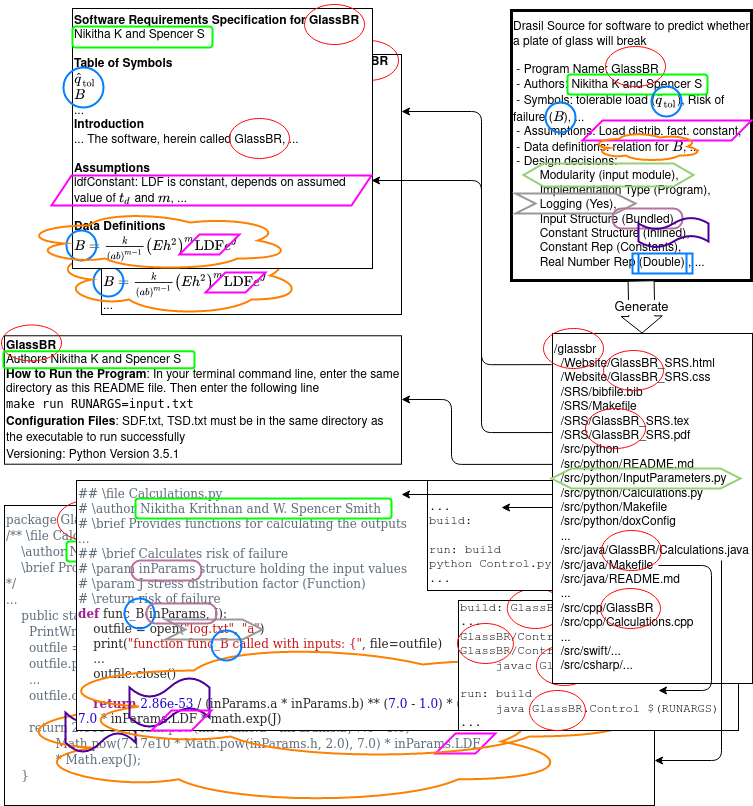
\includegraphics[width=\linewidth]{assets/DrasilSupportsChange-right-portrait-overlapped-ungrouped-v1.drawio.png}
  \caption{Mapping between changes in DSL source code to the generated
  artifacts. The different colors and shapes show the connection between the
  source knowledge and the generated artifacts.}
  \Description{Mapping between changes in DSL source code to the generated
  artifacts. The different colours and shapes show the connection between the
  source knowledge and the generated artifacts.}
  \label{Fig_DrasilAndChange}
\end{figure*}

\subsection*{Step 3a: Base Knowledge}

\begin{lstlisting}
  fullyT, glassTypeFac, heatS, iGlass, lGlass :: CI
  fullyT = commonIdeaWithDict "fullyT" (nounPhraseSP "fully tempered") "FT" [idglass]
  glassTypeFac = commonIdeaWithDict "glassTypeFac" (nounPhraseSP "glass type factor") "GTF" [idglass]
  heatS = commonIdeaWithDict "heatS" (nounPhraseSP "heat strengthened") "HS"[idglass]
  iGlass = commonIdeaWithDict "iGlass" (nounPhraseSP "insulating glass") "IG"[idglass]
  lGlass = commonIdeaWithDict "lGlass" (nounPhraseSP "laminated glass") "LG" [idglass]
\end{lstlisting}

\begin{lstlisting}
  risk :: DataDefinition
  risk = ddE riskQD
    [dRef astm2009, dRefInfo beasonEtAl1998 $ Equation [4, 5],
    dRefInfo campidelli $ Equation [14]]
    Nothing "riskFun" [aGrtrThanB, hRef, ldfRef, jRef]
    where riskQD = mkQuantDef riskFun riskEq
          riskEq = (sy sflawParamK $/
            (mulRe (sy plateLen) (sy plateWidth) $^ (sy sflawParamM $- exactDbl 1))) `mulRe`
            ((sy modElas `mulRe` square (sy minThick)) $^ sy sflawParamM) `mulRe` sy lDurFac `mulRe` exp (sy stressDistFac)
\end{lstlisting}

\subsection*{Step 3b: Coherent Narrative}

As per the requirements template for scientific software~\cite{SmithAndLai2005,
SmithEtAl2007}, we have a goal: ``\textbf{Predict-Glass-Withstands-Explosion}: Analyze and predict whether the glass slab
under consideration will be able to withstand the explosion of a certain degree
which is calculated based on user input.'' The goal statement is generated via:

\begin{lstlisting}
willBreakGS :: ConceptInstance
willBreakGS = cic "willBreakGS" (foldlSent [S "Analyze" `S.and_`
S "predict whether the", phrase glaSlab, S "under consideration will be able",
S "to withstand the", phrase explosion `S.of_` S "a certain", phrase degree_',
S "which is calculated based on", phrase userInput])
"Predict-Glass-Withstands-Explosion" goalStmtDom
\end{lstlisting}

\subsection*{Step 4a: Specialization of Theories}

Theories are specialized via assumptions, like this one: ``\textbf{glassCondition}:
Following astm2009 (pg. 1), this practice does not apply to any form of wired,
patterned, etched, sandblasted, drilled, notched, or grooved glass with surface
and edge treatments that alter the glass strength. (RefBy:
UC:Accommodate-Altered-Glass.)''  This assumptions is generated via:

\begin{lstlisting}
glassConditionDesc :: Sentence
glassConditionDesc = foldlSent [S "Following", complexRef astm2009 (Page [1]) `sC` 
  S "this", phrase practice, S "does not apply to any form of", foldlList Comma Options $ map S ["wired",
  "patterned", "etched", "sandblasted", "drilled", "notched", "grooved glass"], S "with", 
  phrase surface `S.and_` S "edge treatments that alter the glass strength"]
\end{lstlisting}

\subsection*{Step 4b: ?}

We create a closed harmonic system containing all related knowledge (in
particular, the grounded theories), which is as simple as collecting them into a
single system.

\begin{lstlisting}
iMods :: [InstanceModel]
iMods = [pbIsSafe, lrIsSafe]

si :: SystemInformation
si = SI {
_sys = glassBR, _kind = Doc.srs, _authors = [nikitha, spencerSmith],
_purpose = purpDoc glassBR Verbose, _quants = symbolsForTable,
_concepts = [] :: [DefinedQuantityDict], _instModels = iMods,
_datadefs = GB.dataDefs, _configFiles = configFp,
_inputs = inputs, _outputs = outputs,
_defSequence = qDefns, _constraints = constrained,
_constants = constants, _sysinfodb = symbMap,
_usedinfodb = usedDB, refdb = refDB
}
\end{lstlisting}

\subsection*{Step 5}

We make choices about the software representations of the theories:

\begin{lstlisting}
code :: CodeSpec
code = codeSpec fullSI choices allMods

choices :: Choices
choices = defaultChoices {
  lang = [Python, Cpp, CSharp, Java, Swift], modularity = Modular Separated,
  impType = Program, logFile = "log.txt", logging = [LogVar, LogFunc],
  comments = [CommentFunc, CommentClass, CommentMod], doxVerbosity = Quiet,
  dates = Hide, onSfwrConstraint = Exception, onPhysConstraint = Exception,
  inputStructure = Bundled, constStructure = Inline, constRepr = Const,
  auxFiles = [SampleInput "../../datafiles/glassbr/sampleInput.txt", ReadME] 
}
\end{lstlisting}

\subsection*{Step 6}

A final executable program which should take the knowledge discussed above, and
use pre-made printers/generators to generate software artifacts, SRS documents,
etc:

\begin{lstlisting}
main :: IO()
main = do
    setLocaleEncoding utf8
    gen (DocSpec (docChoices SRS [HTML, TeX]) "GlassBR_SRS") srs printSetting
    genCode choices code
    genDot fullSI
    genLog fullSI printSetting
\end{lstlisting}

\section{Concluding Remarks} \label{ch:concluding_remarks}

For well understood domains, building software ought to be a matter of
engineering, based on solid scientific foundations. The ultimate test of ``well
understood'' is being able to teach the domain language to a computer. We have
shown samples of a process and implementation framework for generating all of
the software artifacts for (well understood) software, from the natural
knowledge base of the domain.

We take advantage of inherent knowledge duplication between artifacts in a
project, and between projects, by capturing the knowledge once and providing
means to transform that information into all of the views needed within a given
project.  Developers can realize long-term productivity with documentation and
code that are consistent by construction.

Codifying scientific, engineering and computational knowledge is challenging,
but success will completely transform the development of software, and software
families, in well understood domains. Our process will remove human errors from
generating and maintaining documentation, code, test cases and build
environments, since the mundane details are handled by the generator.  With the
new software tools, we can potentially detect inconsistencies between theory via
inter-theory consistency constraints. Moreover, we can explicitly track the
ramifications of a proposed change.  With the right up-front investment, we can
have sustainable software because stable knowledge is separated from rapidly
changing assumptions and design decisions.

%% Bibliography
\bibliographystyle{ACM-Reference-Format}
\bibliography{References}

\end{document}

% Good quotes:
% \begin{itemize}
% \item metaprograms are just programs
% \item models outside an integrated toolchain are insufficiently useful
% \end{itemize}
